\chapter{Gaussian Approximations}

\section*{5.1. Equal percentages}
\addcontentsline{toc}{section}{5.1. Equal percentages}
In the last paragraph of Section 2.1, the same percentage
99.999999975\%, appeared twice. Explain why you know that 
these two percentages must be the same, even if you don't
know what the common value is.

\vspace{1em}

\begin{proof}
    We've seen that for a high number of flips, the binomial 
    distribution reduces to a Gaussian distribution
    with the standard deviation $\sigma = \sqrt{n/4}$. Since we are dealing with a 
    Gaussian distribution, the probability that the number of Heads
    obtained differs from the expected number by at most $\Delta x$ Heads is given
    by the number of standard deviations needed to reach $\Delta x$.
    The two experiments in Section 2.1 were:
    \begin{enumerate}[(i)]
        \item $n_1 = 10^5$ flips and the probability that the expected number of
            Heads differs by more than $\Delta p_1 = 1\%$ of the expected value
            is given by our percentage. Hence, the standard deviation is given by
            $\sigma_1 = \sqrt{10^5 / 4} = 50\sqrt{10}$ and the number of flips
            that deviate from the expected value is $\Delta x_1 = n_1 \Delta p_1 = 10^3$.

        \item $n_1 = 10^5$ flips and the probability that the expected number of
            Heads differs by more than $\Delta p_2 = 0.01\%$ of the expected value
            is given by our percentage. Hence, the standard deviation is given by
            $\sigma_2 = \sqrt{10^9 / 4} = 5000\sqrt{10}$ and the number of flips
            that deviate from the expected value is $\Delta x_2 = n_2 \Delta p_2 = 10^5$.
    \end{enumerate}

    Now, since the number of standard deviations to reach the needed $\Delta x$'s are
    equal for both cases,
    \[
        \frac{\Delta x_1}{\sigma_1} = \frac{10^3}{50\sqrt{10}} = 5 \sqrt{10}
        = \frac{10^5}{5000\sqrt{10}} 
        = \frac{\Delta x_2}{\sigma_2}
    \] 
    we have that the percentage that the number of Heads does not deviate
    from the expected value more than $\Delta x$ Heads is the same for both
    cases, that is 99.999999975.
\end{proof}

\section*{5.2. Rolling sixes}
\addcontentsline{toc}{section}{5.2. Rolling sixes}
In the solution to Problem 2.13 (known as the Newton-Pepys problem), we
noted that the answer to the question, "If $6n$ dice are rolled, what is the
probability of obtaining at least $n$ 6's?", approaches 1/2 in the $n \to \infty$
limit. Explain why this is the case.

\vspace{1em}

\begin{proof}
    We know that for $n \to \infty$ the Binomial distribution reduces to the 
    Gaussian distribution. Let $X$ denote the number of 6's that are obtained 
    in $6n$ rolls. Assuming that the probability of a dice to be rolled as a 6
    is 1/6, we get that $E[X] = n$, i.e. the expected number of 6's after $6n$ 
    rolls is $n$. As $n \to \infty$, the probability
    of obtaining exactly $n$ 6's is negligible, so the probability that we 
    get at least $n$ sixes is roughly given by the area of the right half of the 
    Gaussian approximation. Therefore, for $n \to \infty$ the sought probability approaches 
    $1/2$ (half of the area of a normalized Gaussian).
\end{proof}

\section*{5.3. Coin flips}
\addcontentsline{toc}{section}{5.3. Coin flips}
If you flip 10$^4$ coins, how surprised would you be if the observed percentage
of Heads differs from the expected value of 50\% by more than 1\%? Answer
the same question for 10$^6$ coins. (These numbers are large enough so that
the binomial distribution can be approximated by a Gaussian).

\vspace{1em}

\begin{proof}
    Since the number of flips are large enough, the Binomial distributions are reduced
    to Gaussians. We analyze the two cases separately:
    \begin{enumerate}[(i)]
        \item We start by seeing that, the standard deviation is given by $\sigma_1 = \sqrt{10^4 / 4} = 50$, and
            that $\Delta x_1 = 10^4 \cdot 1\% = 100$. Now, we "shift" the Gaussian so that
            $\mu = 0$. The graph will show us the probabilities of the observed
            value relative to the expected value. Therefore, the probability
            that the observed number of Heads differs from the expected value of
            50\% by more than 1\% is given by:
            \[
                p_1 
                = 1 - \frac{1}{\sqrt{2 \pi {\sigma_1}^2}} 
                    \int_{-\Delta x_1}^{\Delta x_1} e^{-\frac{x^2}{2{\sigma_1}^2}} dx
                = 1 - \frac{1}{50\sqrt{2\pi}} 
                    \int_{-100}^{100} e^{-\frac{x^2}{2 \cdot 50^2}} dx
                \approx 1 - 0.9544 = 0.0455 = 4.55\%
            \] 

        As a result, I would be surprised, but not very much so. 4.55\% is not a big percentage, but 
        certainly not negligible.

    \item Analogously with the other case, we have that $\sigma_2 = \sqrt{10^6/4} = 500$ and 
        $\Delta x_2 = 10^6 \cdot 1\% = 10^3$. By "shifting" the Gaussian again such that
        $\mu = 0$, the probability that the observed number of Heads differs from
        the expected value of 50\% by more than 1\% is:
        \[
            p_2 
            = 1 - \frac{1}{\sqrt{2 \pi {\sigma_2}^2}} 
                \int_{-\Delta x_2}^{\Delta x_2} e^{-\frac{x^2}{2{\sigma_2}^2}} dx
            = 1 - \frac{1}{500\sqrt{2}} 
                \int_{-10^3}^{10^3} e^{-\frac{x^2}{2 \cdot 500^2}} dx
            \approx 0 \approx 0\%
        \] 

        Therefore, I would be extremely surprised by the result, as this occuring seems 
        very close to impossible.
    \end{enumerate}
\end{proof}

\section*{5.4 Identical distributions}
\addcontentsline{toc}{section}{5.4. Identical distributions}
A thousand dice are rolled. Fig. 5.15 shows the probability distribution (given
by Eq. (5.15)) for the number of 6's that appear, relative to the expected number
(which is 167). How many $\emph{coins}$ should you flip if you want the probability
distribution for the number of Heads that appear (relative to the expected number)
to look exactly like the distribution in Fig. 5.15 (at least in the Gaussian
approximation)?

\begin{figure}[H]
    \center{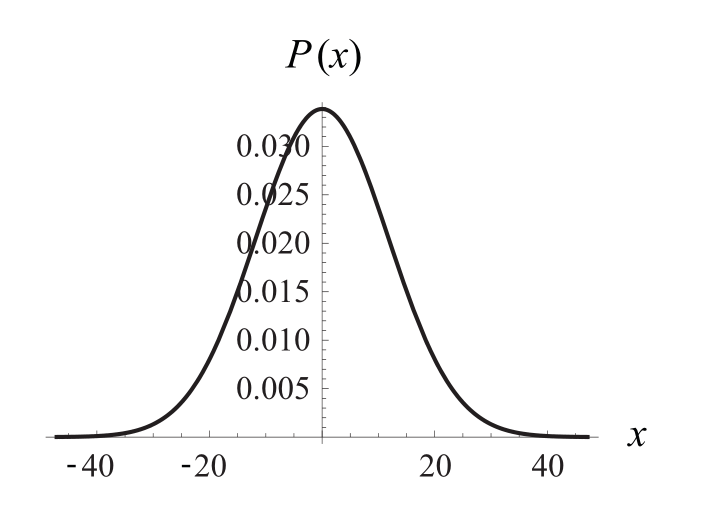
\includegraphics[width=0.6\linewidth]{figure5_15.png}}
    \caption*{\textbf{Figure 5.15}: The probability distribution for the number of 6's in 1000
    dice rolls, relative to the expected number, 167.}
\end{figure}

\vspace{1em}

\begin{proof}
    Both the dice and coin distributions are binomial distributions, so we'll approximate
    them as Gaussian distributions. A Gaussian distribution is uniquely identified by its
    mean and standard deviation, so two distributions are identical if they have these
    two attributes identical. Since we are interested by the distribution 
    for the number of Heads relative to the expected number, we don't care about the mean.
    Therefore, the standard deviation of the dice distribution must be the same as the one
    of the coin distribution. Knowing that the standard deviation for a Gaussian approximation
    of a binomial distribution is given by $\sqrt{np(1 - p)}$, and by considering fair coins/dice,
    we notice that the standard deviations of the distributions are equal for:
    \[
        \sqrt{1000 \cdot \frac{1}{6} \cdot \frac{5}{6}} = \sqrt{\frac{n}{4}} 
        \iff \frac{50\sqrt{2}}{6} = \frac{\sqrt{n}}{2}
        \iff 50\sqrt{2} = 3\sqrt{n} \iff n = \frac{5000}{9} \approx 556
    \] 

    Therefore, we need to flip 556 coins to obtain a very close Gaussian distribution to
    Fig. 5.15.
\end{proof}

\section*{5.5. Gambler's fallacy}
\addcontentsline{toc}{section}{5.5. Gambler's fallacy}
Assume that after 20 coin flips, you have obtained only five Heads. The
probability of this happening is small (about 1.5\%, since $\binom{20}{5} / 2^{20} = 0.0148$),
but not negligible. Since the law of large numbers says that the fraction of Heads approaches
50\% as the number of flips gets large, should you expect to see more Heads and Tails in
future flips?

\vspace{1em}

\begin{proof}
    Since coin flips are independent events, we can't make any assumption about future flips
    based on the already done 20 flips. Also, we can't assume anything based on the law of large
    numbers, since it assumes that the number of trials goes to infinity, so any unusual trends could
    occur at any time, and their effect will be diminished as the number of trials increases. 
\end{proof}

\section*{5.6. Finding the Gaussian}
\addcontentsline{toc}{section}{5.6. Finding the Gaussian}
What is the explicit form of the Gaussian function $f(x)$ that matches
up with the fourth histogram in Fig. 5.11? Assume that $n_t = 10$ is large
enough so that the Gaussian approximation does indeed hold.

\begin{figure}[H]
    \center{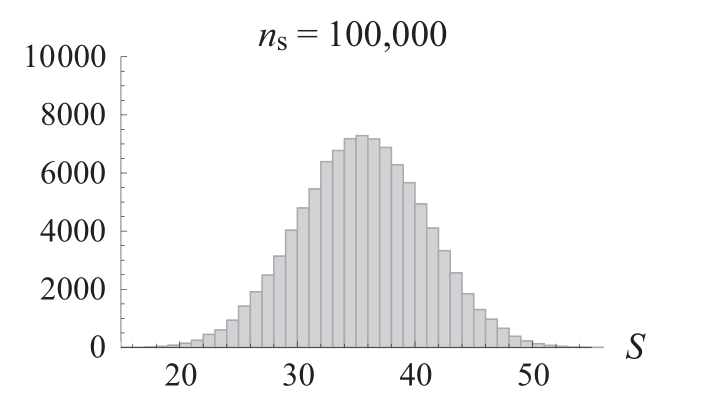
\includegraphics[width=0.6\linewidth]{figure5_15_histogram.png}}
    \caption*{\textbf{Figure 5.11}: Fourth Histogram}
\end{figure}

\vspace{1em}

\begin{proof}
    We assume that $n_t = 10$ is large enough so the Gaussian approximation holds.
    Let $X$ denote the outcome of a dice roll and let $Y$ represent the sum of 10 such outcomes,
    so $Y = X_1 + X_2 + \ldots X_{10}$, where the $X_i$s are distributed the same as $X$.
    One can easily show that $\sigma_X = 1.71$ and $\mu_X = 3.5$. The mean of $Y$ is easily
    obtained by using the linearity of expectation:
    \[
        \mu_Y = E[Y] = E\bigg[\sum_{i = 1}^{10}X_i\bigg] = 10E[X] = 10\mu_X = 35
    \] 

    The variance of $Y$ is computed by also using the fact that the $X_i$ variables
    are independent, so the expectation of their product can be split:
    \begin{align*}
        {\sigma_Y}^2 
        = E[Y^2] - {\mu_Y}^2 
        &= E\bigg[\bigg(\sum_{i = 1}^{10} X_i\bigg)^2\bigg] - 100\mu_X^2 
        = 10E[X^2] + 2\sum_{i = 1}^{10}\sum_{j = i + 1}^{10} E[X_i X_j] - 100\mu_X^2 \\
        &= 10E[X]^2 - 110\mu_X^2 + 10\mu_X^2 
        = 10E[X]^2 - 10\mu_X^2 = 10\sigma_X^2 \approx 29.24
    \end{align*}

    From the Central Limit Theorem, we know that $Y$ will be the Gaussian approximation 
    of the process described by the histogram. Therefore, since the probabilities
    represent the number of sums with a specific value (height of the columns), divided
    by the number of total sums ($n_s$), the Gaussian function associated to the histogram
    is given by the PDF of $Y$, scaled by $n_s$:
    \[
        f(x) = n_s G(y | \mu_Y, \sigma_Y^2) 
        = \frac{10^5}{29.24\sqrt{2\pi}} e^{-\frac{(y - 35)^2}{2\cdot 29.24^2}}
    \] 
\end{proof}

\section*{5.7. Standard deviations}
\addcontentsline{toc}{section}{5.7. Standard deviations}
Calculate the theoretically predicted standard deviations of the histograms in
Figs. 5.13 and 5.14, and check that your results are consistent with a visual
inspection of the histograms. You will need the result from Problem 4.3 for
Fig. 5.14.

\vspace{1em}

\begin{proof}
    We analyze the two figures separately:

    \vspace{1em}

    \textbf{Fig. 5.13} The histogram shows the result of taking $n_s = 10^5$ averages of
    $n_t = 100$ numbers chosen from the distribution in Fig. 5.12. Let $X$ be a
    random variable modeled by the distribution in Fig. 5.12. Then,
    \[
        P(X = 2) = 0.6 \hspace{2em} P(X = 3.1) = 0.1 \hspace{2em} P(X = 7) = 0.3
    \] 

    Therefore, the mean of $X$ is 
     \[
         \mu_X = E[X] = 2 \cdot 0.6 + 3.1 \cdot 0.1 + 7 \cdot 0.3 = 3.61
    \] 
    while the variance is given by
    \[
        \sigma_X^2 = E[(X - \mu)^2] = (2 - 3.61)^2 \cdot 0.6 + (3.1 - 3.61)^2 \cdot 0.1 + (7 - 3.61)^2 \cdot 0.3 
        \approx 5.26
    \] 

    Now, let $Y$ denote the average of $100$ numbers distributed like $X$ (denoted by $X_i$), so
    \[
        Y = \frac{1}{100}\sum_{i = 1}^{100} X_i
    \] 

    By using the linearity of expectation, the mean of $Y$ is
    \[
        \mu_Y = E[Y] = \frac{1}{100}E\bigg[\sum_{i = 1}^{100} X_i\bigg] 
        = \frac{1}{100}\sum_{i = 1}^{100} E[X_i] 
        = E[X] = \mu_X = 3.61
    \] 

    and the variance is given by:
    \[
        \text{Var}(Y) = \text{Var}\bigg(\frac{1}{100} \sum_{i = 1}^{100} X_i\bigg)
        = \frac{1}{10^4} \text{Var}\bigg(\sum_{i = 1}^{100} X_i\bigg)
        = \frac{1}{10^4} \sum_{i = 1}^{100} \text{Var}(X_i)
        = \frac{1}{100} \text{Var}(X) = 0.0526
    \]
    which gives the standard deviation:
    \[
        \sigma_Y \approx 0.23
    \] 

    \begin{figure}[H]%
        \centering
        \subfloat[\centering Histogram in Fig 5.13]{{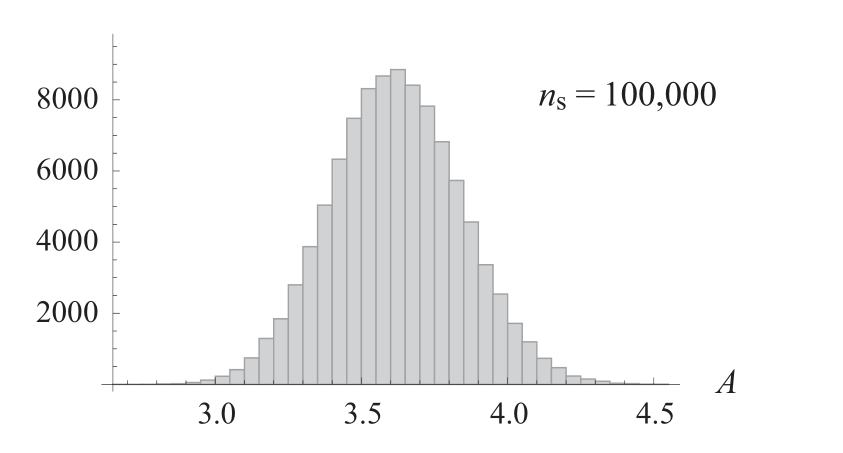
\includegraphics[width=0.49\linewidth]{5_7_fig513.png} }}%
        \qquad
        \subfloat[\centering Gaussian with $\mu = 3.61, \sigma = 0.23$, scaled by $10^5$]{{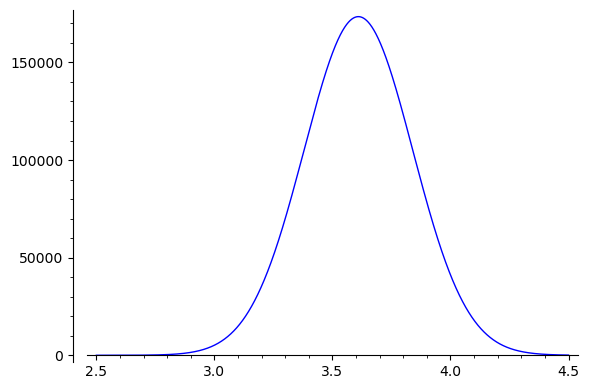
\includegraphics[width=0.44\linewidth]{5_7_gauss2.png} }}%
    \end{figure}

    \vspace{1em}

    \textbf{Fig. 5.14.} The histogram portrays the results of taking $n_s = 10^5$ averages
    of $n_t = 50$ numbers chosen from a uniform distribution (from 0 to 1). Let X be
    distributed by that uniform distribution. The mean of the uniform distribution 
    is just $\mu_X = 1/2$ and the variance is given by the result from Problem 4.3, i.e.
    $\sigma_X^2 = 1/12$. Now, let $Y$ denote the average of 50 numbers chosen from this
    distribution, so basically
    \[
        Y = \frac{1}{50} \sum_{i = 1}^{50} X_i
    \] 
    where the $X_i$ variables are distributed like $X$.
    If we assume that $n_t = 50$ is large enough for the Central Limit Theorem to apply,
    we find that $Y$ is modeled by a Gaussian distribution. Note that the 1/50 scaler
    does not change this, because a scaled Gaussian is still a Gaussian. Therefore, by
    using the linearity of expectation, we get the mean of $Y$:
    \[
        \mu_Y = E[Y] = \frac{1}{50}E\bigg[\sum_{i = 1}^{50} X_i\bigg] 
        = \frac{1}{50}\sum_{i = 1}^{50} E[X_i] 
        = E[X] = \mu_X = \frac{1}{2}
    \] 

    Similarly, by using the fact that the variance of a sum of random variables is equal
    to the sum of variances (for independent variables), we have that:
    \[
        \text{Var}(Y) = \text{Var}\bigg(\frac{1}{50} \sum_{i = 1}^{50} X_i\bigg)
        = \frac{1}{50^2} \text{Var}\bigg(\sum_{i = 1}^{50} X_i\bigg)
        = \frac{1}{50^2} \sum_{i = 1}^{50} \text{Var}(X_i)
        = \frac{1}{50} \text{Var}(X) = \frac{1}{600}
    \] 
    which gives the standard deviation
    \[
        \sigma_Y = \frac{1}{10\sqrt{6}}
    \] 

    We can confirm that this result is valid by comparing the plot of the corresponding Gaussian 
    function in the figure with the histogram and seeing that they are are very similar: 
    \begin{figure}[H]%
        \centering
        \subfloat[\centering Histogram in Fig 5.14]{{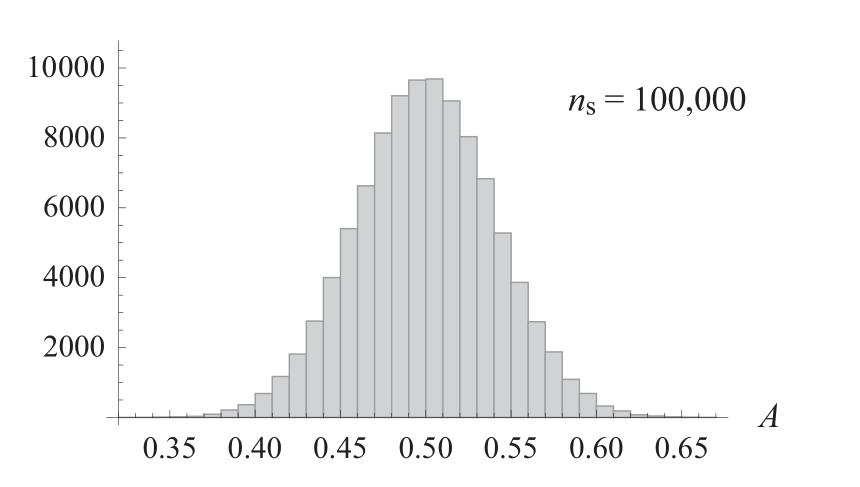
\includegraphics[width=0.49\linewidth]{5_7_fig514.png} }}%
        \qquad
        \subfloat[\centering Gaussian with $\mu = 1/2, \sigma = \frac{1}{10\sqrt{6}}$, scaled by $10^5$]{{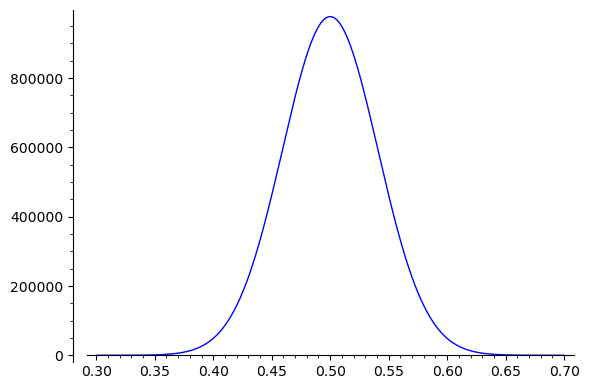
\includegraphics[width=0.44\linewidth]{5_7_gauss1.png} }}%
    \end{figure}
\end{proof}
